In this work, we evaluate three kinds of programs for energy auto-tuning with
polyhedral framework: Polybench programs, publicly-accessible LULESH 
program\cite{LULESH:versions}, and a realistic application developed and frequently 
used by our collaborators.

\subsection{Polybench}
Previous work has obtained significant speedups with the 
polyhedral framework for the Polybench programs\cite{EJ2011,EJ2012,EJ2013}.
Extending that work to examine whether the best tuned variants are also
the most energy efficient is the focus of this work.
Using PoCC, program variants were generated using
a different set of the 
optimizations from the following five groups: 
\begin{itemize}
    \item Loop fusion: smartfuse, maxfuse, nofuse
    \item Loop unrolling factor: 1, 2, 4, 8
    \item Loop tiling: 1, 16, 32, 64. Note that the number of different flags
 depends on the level of nested loops   
    \item Loop vectorization: on, off
    \item Loop parallelization: on, off
\end{itemize}
%\WW{We rely on Tiling Hyperplane method\cite{Hyperplane} to legally perform loop
%transformations. Loop fusion is performed to maximize locality by fusing statements. 
%As in\cite{EJ2013}, 1) nofuse means we do not fuse statements at all;
% 2)smartfuse means we only fuse together statements that carry data reuse and of 
%similar loop nesting depth; 3) maxfuse means we maximally fuse statements.
% }
The Tiling Hyperplane method\cite{Hyperplane} is used to legally perform loop transformations.
Loop fusion is performed to minimize loop overheads. Depending on reuse patterns, fusion can increase or decrease locality. As in\cite{EJ2013}, 1) nofuse results in no loop fusion 2) smartfuse only
fuses statements that carry data reuse and are at similar nesting levels 3) maxfuse performs all legal loop fusion.
If the maximum nested loop level is 3, applying all possible combinations
of the above flags generates 5135 program variants. The ROSE source-to-source
compiler was used to add energy profiling calls to each variant.
GCC(4.4.6) generated the final executable. During execution,
 periodic queries to the RCRtool blackboard provide the energy consumption information.
Figure~\ref{fig:Workflow} gives the workflow for measuring energy consumption of 
Polybench programs using the energy-aware polyhedral compiler framework.

\begin{figure}[t]
    %\rotatebox{-90}{\includegraphics[height=3in]{TE}}
    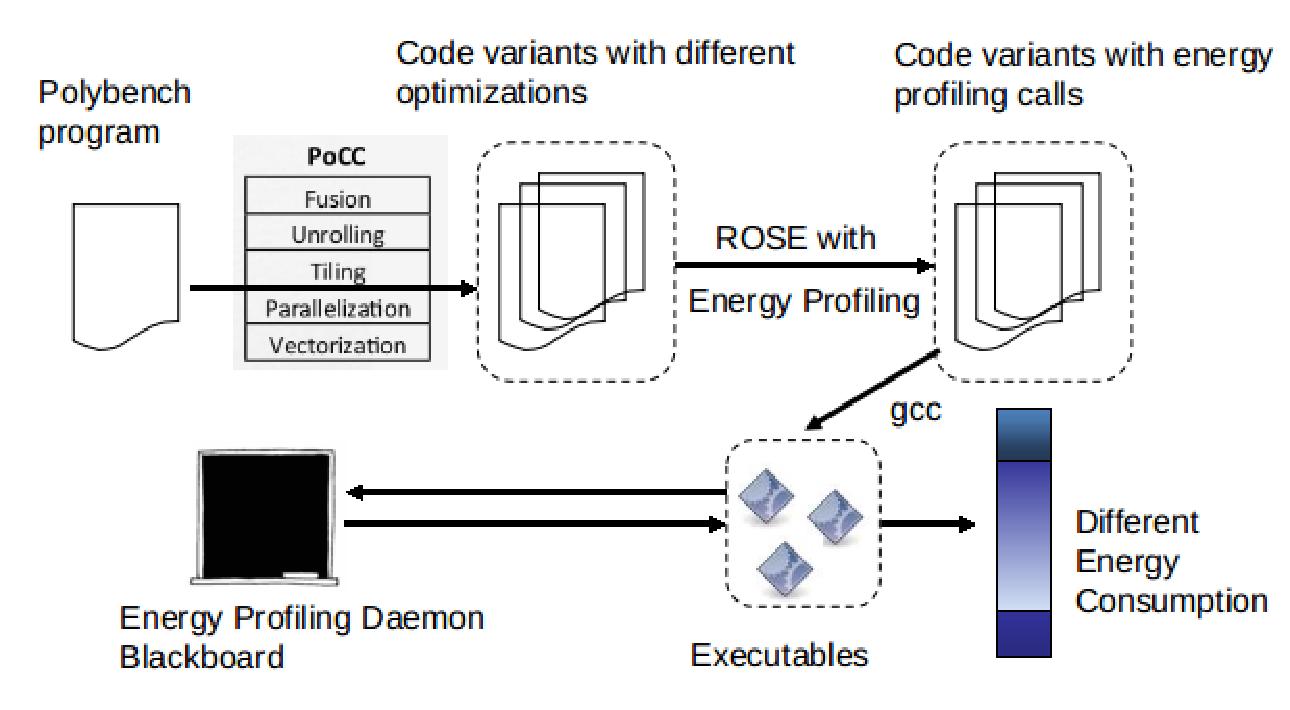
\includegraphics[width=3.4in]{workflow}
    \caption{Graph showing the workflow of obtaining energy consumption of polyhedral
optimized (Polybench) programs. }
    \label{fig:Workflow}
\end{figure}

\subsection{LULESH}
LULESH\cite{LULESH:versions} is a shock hydrodynamic simulation application. It
mimics a larger realistic application called ALE3D. We used the OpenMP implementation
v1.0 for evaluation. The original LULESH uses a 
block structured mesh accessed via an indirect reference pattern\cite{LULESH:versions}.
%In order to make LULESH go through the polyhedral compilation procedure, we modified
To make LULESH go through the polyhedral compilation procedure, we modified
LULESH by resolving all indirect array accesses. Although doing this oversimplified
LULESH, it allows us to study the energy and time relationship of polyhedral 
compilation techniques with LULESH. 

LULESH OpenMP implementation contains 30 parallel regions, 6 of which take up more
than $60\%$ of the total application time\cite{us}. We manually converted two most 
significant parallel regions to two SCoPs so that they can be passed to polyhedral
framework. The resulting largest SCoP contained too many dependences and we found
it was hard for the polyhedral compiler to finish transformation and parallelization.
When all temporary variables were eliminated from the most computationally intensive loop
to create an SCoP, greatly expanded statements required hours of compilation to finish generating even one variant.
%Even when all the dependences are eliminated inside the largest SCoP, it still took the polyhedral
%compiler hours to finish one transformation.
In this work, we focus on optimizing 
the 2nd (largest) SCoP of LULESH. 200 program variants were produced 
by applying loop fusion (maxfuse and 
smartfuse), loop tiling, vectorization, and parallelization.
The execution time and energy of each was measured.

\subsection{A Realistic Application}
In addition to the Polybench programs, a 2D monodomain cardiac wave propagation simulation 
(named \emph{brdr2d}) was used as a test case. Its model involves
solving a set of ODEs and PDEs and is well-known in the computational 
cardiac modeling field\cite{Me}. Equation (1) is the PDE that needs to be 
solved. The ODEs are used to represent the $I_{ion}$ variable.
\begin{equation}
C_{m}\frac{\partial V_{m}}{\partial t} = \nabla \cdot D\nabla{V_{m}}-I_{ion}
\end{equation}
The sequential C implementation is more than 1K lines. 

One loop nest takes up more than 90\% of the total application execution time. 
The dominate loop nest is an ideal situation for the polyhedral compiler. 
The loop nest is inside a while loop and is executed many times. 
This code structure is not unique to cardiac wave propagation simulation. 
Computationally dominate loops inside either while loops looking for 
some termination condition or inside a simulation time-step loop
are common in scientific codes. LULESH falls into this category
with multiple loop nests within a time-step loop.

While PolyOpt originally cannot extract any SCoP from \emph{brdr2d}, it does output
information useful to the user to manually transform the application to contain at least one SCoP.
To expose the SCoPs the following changes were required. The computation part 
of \emph{brdr2d} was fully inlined removing all function calls.
Then, all array indexes were changed to be affine functions of the 
loop iterators. This involved loop unswitching to specialize modular operations
like $step~\%~2$. Finally, the number of dependencies was reduced by forward substitution
of temporary variables. After these changes, PolyOpt automatically detected the code
region and applied various transformations to the SCoPs. 

%Different from LULESH, the forward substitution did not result in 
%extreme expansion of code when converting the nested loops into SCoPs. Thus, the 
%polyhedral compiler generated program variants in a timely manner.

Program variants were generated to explore data locality and parallelism
using loop fusion (smartfuse/maxfuse), different tiling sizes, vectorization and auto-parallelization. 
OpenMP pragmas were automatically generated for each variant.
%The original sequential C implementation had OpenMP pragmas manually added to serve as
The original sequential C implementation had all required OpenMP pragmas manually added to serve as
a baseline.
Four different input files for \emph{brdr2d} were used to study how the
performance of the program variants is impacted by different
input sizes. 
 
